\documentclass[10pt]{article}
\usepackage[utf8]{inputenc}
\usepackage[T1]{fontenc}
\usepackage{amsmath}
\usepackage{amsfonts}
\usepackage{amssymb}
\usepackage[version=4]{mhchem}
\usepackage{stmaryrd}
\usepackage{graphicx}
\usepackage{pdfpages}


\title{Problem Set 2 }


\author{Applied Math 205, Fall 2024}
\date{}


\begin{document}
\maketitle
Due as a pdf file on Gradescope before 3:00 pm, Monday 30 September
\emph{I used ChatGPT to help me here.}
\section{}
Low-rank approximation of Old Glory. On Canvas, you will find two files flag1.jpg and flag2.jpg, each with a color image of the United States flag. Adapt the code p6\_iterativeGE.m from the Sept. 16 lecture, or its Python equivalent, to produce low-rank approximations of monochrome versions of these images by Gaussian elimination with complete pivoting. As always in AM205, be sure to list your code.

Run your code to produce a plot of 9 images corresponding to approximations of image 1 of ranks \(k=1,2,4, \ldots, 256\). Also, produce a plot of the root-mean-square error in the low-rank approximation as a function of \(k\) (all values of \(k\), not just powers of 2). Then do all this again for image2. Comment on the results, and in particular on the comparison between the two images. Why does one series converge faster than the other?\\
\subsection{}
The low-rank approximation for the first image converges faster; this is expected because it is simpler and has more structure, which are things that can be taken advantage of by a low-rank approximation, as indicated by the faster convergence in RMSE.
\section{}
2. Least-squares fitting by ellipses. Suppose we have $m$ data points $\left(x_{1}, y_{1}\right), \ldots,\left(x_{m}, y_{m}\right)$ in the $x-y$ plane and we want to find an ellipse that fits them well. Finding the geometrically closest fit is a nonlinear problem, but we can come close by a linear formulation. An equation for an ellipse centered at $(0,0)$ is

$$
b x^{2}+c x y+d y^{2}=1
$$

Let us view $b, c$ and $d$ as unknowns and find them by solving a linear least-squares problem.\\
\subsection{}
(a) Write down in matrix form an $m \times 3$ least-squares problem whose unknown vector is $(b, c, d)^{T}$.\\
\subsubsection{}
The least-squares problem is given by the following matrix equation:
\begin{equation}
  \begin{bmatrix}
    x_{1}^{2} & x_{1} y_{1} & y_{1}^{2} \\
    x_{2}^{2} & x_{2} y_{2} & y_{2}^{2} \\
    \vdots & \vdots & \vdots \\
    x_{m}^{2} & x_{m} y_{m} & y_{m}^{2} \\
  \end{bmatrix}
  \begin{bmatrix}
    b \\
    c \\
    d \\
  \end{bmatrix}
  =
  \begin{bmatrix}
    1 \\
    1 \\
    \vdots \\
    1 \\
  \end{bmatrix}
\end{equation}
This matrix equation is merely an extension of the ellipse equation to the $m$ data points.
\subsection{}
(b) Write a function $[b, c, d]=$ ellipse ( $\mathrm{x}, \mathrm{y}$ ) which uses " " to solve this problem. Write driver code to call ellipse for the data

$$
(3,3),(1,-2),(0,3),(-1,2),(-2,-2),(0,-4),(-2,0),(2,0)
$$

print $b, c, d$ and also plot the data points and the fitting ellipse. (Hint: you may find it helpful to take a range of angles $\theta$ and work with corresponding ratios $y / x=\tan \theta$.)\\
For fun (but not to hand in) you might enjoy fitting ellipses to points input interactively with the mouse. In Matlab you can do it like this:

\begin{verbatim}
hold off, axis([-3 3 -3 3 3 $]$, axis manual, hold on, grid on
$\mathrm{x}=[] ; \mathrm{y}=[] ;$ button = 1;
disp('input points with mouse, button >= 2 for final point')
while button == 1
    [xx,yy,button] = ginput(1)
    $\mathrm{x}=[\mathrm{x} ; \mathrm{xx}] ; \mathrm{y}=[\mathrm{y} ; \mathrm{yy}] ; \mathrm{plot}\left(\mathrm{xx}, \mathrm{yy}, \mathrm{xb}^{\prime}\right)$
end
\end{verbatim}
\section{}
Least-squares solution of the Laplace equation. Consider the Laplace equation $\partial^{2} u / \partial x^{2} + \partial^{2} u / \partial y^{2} = 0$ on the unit disk $x^{2} + y^{2} \leq 1$, with boundary data $f(x, y)$. Equivalently, one could think in polar coordinates, $x = r \cos (\theta)$ and $y = r \sin (\theta)$.\\
Solve this problem numerically with the boundary data $f(x, y) = \sqrt{(x - 1.1)^{2} + y^{2}}$ by the following method. Discretize the unit circle by $m = 1000$ equally spaced points, and let $n$ be a small integer. Make an $m \times (2n + 1)$ matrix $A$ whose columns correspond to discretizations of the functions (each of which satisfies the Laplace equation)

$$
1, r \cos (\theta), r \sin (\theta), r^{2} \cos (2 \theta), r^{2} \sin (2 \theta), \ldots, r^{n} \cos (n \theta), r^{n} \sin (n \theta)
$$

Now solve a least-squares problem involving $A$ to fit the given function $f$ on the unit circle by a linear combination of these functions, and evaluate the result to estimate the solution value $u(x = 0.8, y = 0.2)$. What numbers do you get for $n = 0, 2, 4, \ldots, 20$? What do you think is the exact solution $u(0.8, 0.2)$ to 4 digits of accuracy?
\subsection{}
The numbers I get are shown by the print out of the notebook. I think that the exact solution to 4 digits of accuracy is 0.4957.

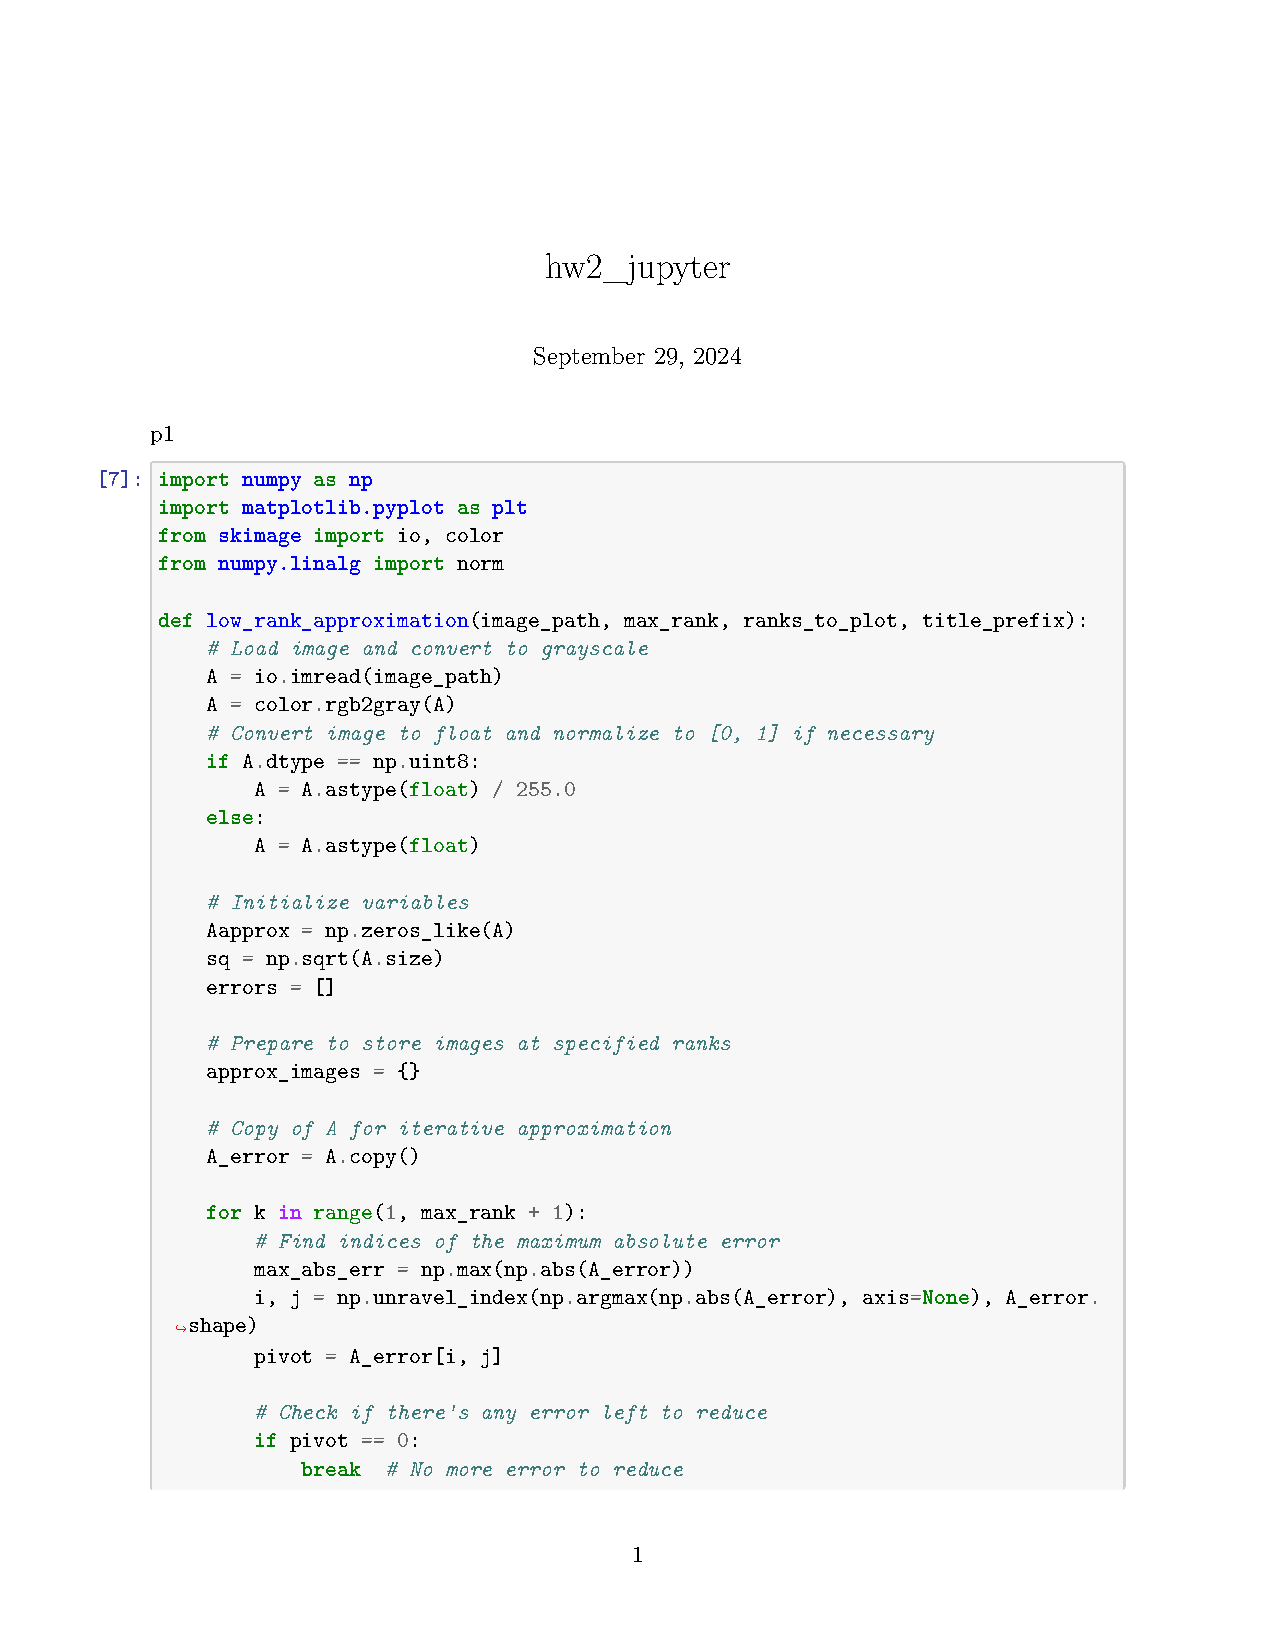
\includepdf[pages=-]{hw2_jupyter.pdf}



\end{document}